\section{Идентифицируемость}
\label{sec:ident}

Первое, что спросит любой, кто это читает: из одноточечного измерения наблюдается ровно скаляр $I(C_0)$,
а параметров в \eqref{eq:theta} три. Тройка $(\pi, E, h)$ точечно не идентифицируется --- любая кривая,
проходящая через ту же ординату при $C_0$, объясняет данные одинаково хорошо.

Риск конкретный: сеть сбросит остаток в $E$, чтобы подогнать показание скрининга, и испортит $\pi$ ---
единственную величину, которую с неё спрашивают на лидерборде.

Что с этим делаем, по возрастанию силы ограничения.

\subsection{Крутизна --- на уровень фермента}

$h_e$, один скаляр на фермент вместо десятков тысяч. Первую версию делаем вообще с $h_e \equiv 1$.
Оправдание не только техническое: крутизна кривой в такой пробе определяется в основном механизмом
и стехиометрией связывания, а не индивидуальными особенностями лиганда, и подгонка калибровки
(раздел~\ref{sec:calib}) даёт по ферментам устойчивые 1.11--1.97.

\subsection{Глубина: амортизация вместо поштучной подгонки}

Есть два способа получить $E$ для каждого соединения.

\emph{Поштучная подгонка}: у каждого соединения свой свободный параметр $E_m$. Для 4905 соединений
и четырёх ферментов это 19\,620 свободных чисел, каждое подбирается только по данным своего соединения,
и никакой связи между похожими молекулами нет.

\emph{Амортизация}: свободных $E_m$ нет вовсе, есть одна общая функция --- голова сети, получающая
представление молекулы и выдающая ответ:
\begin{equation}
E_{m,e} = \sigma\bigl(u_e^{\top} z_m + c_e\bigr) .
\label{eq:eamort}
\end{equation}

Здесь $z_m$ --- вектор-представление молекулы из общего ствола, $u_e$ и $c_e$ --- веса и сдвиг головы
фермента, сигмоида зажимает ответ в интервал от нуля до единицы. Параметров $4(d+1)$, то есть при $d=256$
чуть больше тысячи, и они обслуживают все соединения сразу, включая те, у которых своей кривой нет.
Отсюда слово: дорогая процедура вывода амортизуется по всем объектам.

Как это работает регуляризатором. Чтобы выдать одному соединению нестандартное
$E$, сети надо сдвинуть его представление, а представление производится общим стволом из структуры, и тот же
ствол обслуживает все похожие молекулы. Подогнать $E$ индивидуально можно только там, где есть структурная
закономерность --- класс молекул, систематически ведущий себя как частичный ингибитор. Если такого класса
нет, а есть только шум подгонки кривой, сети выгоднее выдать всем примерно одинаковое $E$. Формально это
сужение множества гипотез: достижимые наборы $\{E_m\}$ --- уже не произвольный вектор длины $N$, а образ
структурного пространства под гладким отображением. Регуляризация здесь не слагаемое в функции потерь,
а свойство параметризации.

\subsection{А теперь измерения, и они меняют вывод}

Всё сказанное объясняет, почему амортизация безопасна. Но у организаторов опубликованы измеренные $E$:
колонки \texttt{EmaxVsPosCtrl\_direct\_inhibition} с доверительными полосами. Смотреть на них надо было
до всяких рассуждений.

\begin{figure}[htbp]\centering
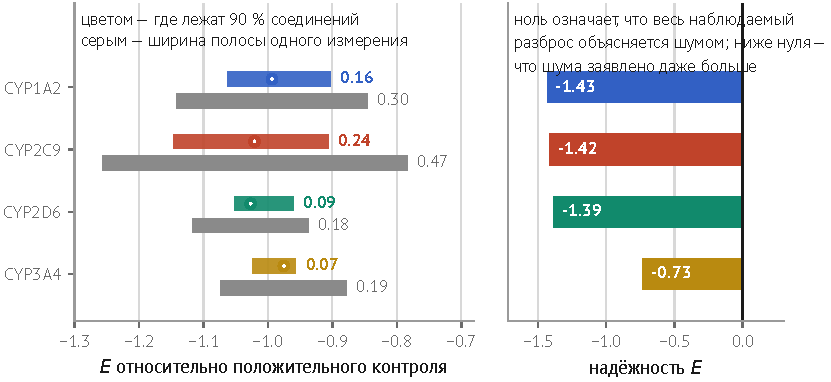
\includegraphics{fig/emax}
\caption{Слева: цветной отрезок --- где лежат 90 процентов соединений, серый --- средняя ширина
доверительной полосы одного измерения. Серый шире цветного на всех четырёх ферментах. Справа: надёжность
по \eqref{eq:rel}, отрицательная везде.}
\label{fig:emax}
\end{figure}

Шкала здесь относительно положительного контроля, поэтому полный ингибитор даёт примерно $-1$.
И вот что оказалось. Весь разброс $E$ \emph{между соединениями} уже, чем заявленная погрешность
\emph{одного} измерения, --- на CYP3A4 втрое, на CYP2D6 вдвое. Иначе говоря, если взять два
случайных соединения, разница их измеренных $E$ в среднем меньше, чем неопределённость каждого
из этих двух чисел по отдельности. Различать соединения по $E$ в такой ситуации нельзя.

Отсюда отрицательная надёжность: от $-0.73$ до $-1.43$. У честной величины она лежит между нулём и единицей;
отрицательная означает, что заявленная дисперсия шума больше всего наблюдаемого разброса. Буквально это
может означать, что полосы посчитаны консервативно, но верхняя оценка сигнала уровня соединения от этого
не меняется --- он не превышает нуля.

Значит амортизация была правильным решением по неправильной причине. Дело не в том, что сеть не
сможет переобучиться на индивидуальные $E$, а в том, что переобучаться там не на чем: сигнала
уровня соединения в этих колонках нет. Вместо головы достаточно одной константы на фермент,
примерно $-1$ у всех четырёх, --- и, если хочется страховки, поштучной поправки с жёстким
штрафом, которую данные обязаны прижать к нулю.

Что наблюдаемая вариация $E$ --- артефакт подгонки кривой, а не химия, видно ещё и по такому
признаку. Связь между измеренным $E$ и активностью почти отсутствует у неактивных и у
активных соединений, но резко усиливается \emph{в средней зоне} --- ровно там, где кривая
доза--эффект обрывается, не дойдя до плато, и подгонщику приходится выбирать глубину
наугад, по гребню. Само по себе это подозрительно. Но решает дело знак: у трёх ферментов
в средней зоне более потентные соединения выглядят давящими \emph{глубже}, а у CYP2D6 ---
наоборот, \emph{мельче}. Химического механизма, который переворачивал бы этот знак от
фермента к ферменту, не существует. Это подпись процедуры подгонки, а не свойство молекул.

Диагностика на будущее остаётся прежней: смотреть разброс выхода головы $E$ отдельно на соединениях
с полной кривой и на соединениях только со скринингом. Если на вторых разброс заметно выше, голова
используется как свалка для остатка.
